%% 
%% Copyright 2007-2019 Elsevier Ltd
%% 
%% This file is part of the 'Elsarticle Bundle'.
%% ---------------------------------------------
%% 
%% It may be distributed under the conditions of the LaTeX Project Public
%% License, either version 1.2 of this license or (at your option) any
%% later version.  The latest version of this license is in
%%    http://www.latex-project.org/lppl.txt
%% and version 1.2 or later is part of all distributions of LaTeX
%% version 1999/12/01 or later.
%% 
%% The list of all files belonging to the 'Elsarticle Bundle' is
%% given in the file `manifest.txt'.
%% 

%% Template article for Elsevier's document class `elsarticle'
%% with numbered style bibliographic references
%% SP 2008/03/01
%%
%% 
%%
%% $Id: elsarticle-template-num.tex 168 2019-02-25 07:15:41Z apu.v $
%%
%%
\documentclass[preprint,12pt]{elsarticle}

%\usepackage{biblatex}
\usepackage{hyperref}
\usepackage{xargs}
\usepackage[colorinlistoftodos,prependcaption,textsize=tiny]{todonotes}

%\usepackage{float,rotating,subfigure}
%\newcommandx{\commentPaul}[2][1=]{\todo[linecolor=red,backgroundcolor=red!25,bordercolor=red,#1]{#2}}
%% Use the option review to obtain double line spacing
%% \documentclass[authoryear,preprint,review,12pt]{elsarticle}

%% Use the options 1p,twocolumn; 3p; 3p,twocolumn; 5p; or 5p,twocolumn
%% for a journal layout:
%% \documentclass[final,1p,times]{elsarticle}
%% \documentclass[final,1p,times,twocolumn]{elsarticle}
%% \documentclass[final,3p,times]{elsarticle}
%% \documentclass[final,3p,times,twocolumn]{elsarticle}
%% \documentclass[final,5p,times]{elsarticle}
%% \documentclass[final,5p,times,twocolumn]{elsarticle}

%% For including figures, graphicx.sty has been loaded in
%% elsarticle.cls. If you prefer to use the old commands
%% please give \usepackage{epsfig}

%% The amssymb package provides various useful mathematical symbols
\usepackage{amssymb}
\usepackage{here}
\graphicspath{{../}{../Figures/}}

%% The amsthm package provides extended theorem environments
%% \usepackage{amsthm}

%% The lineno packages adds line numbers. Start line numbering with
%% \begin{linenumbers}, end it with \end{linenumbers}. Or switch it on
%% for the whole article with \linenumbers.
%% \usepackage{lineno}

\usepackage{gensymb}
\usepackage{amsmath}


\journal{Solar Energy}

\setlength{\marginparwidth}{2cm}
\begin{document}

%\begin{frontmatter}


\title{Annual Antireflection Solar Module Enhancements for Fixed Modules}
%\title{Antireflection Solar Module Enhancement}



\author{Sooraj P. Sharma_1}

\address{\textsuperscript{1}University of Pittsburgh, Department of Mechanical and Materials Science, Pittsburgh, PA 15261, USA}

\author{Paul W. Leu_{1,2,3,*}}
\address{\textsuperscript{1}University of Pittsburgh, Department of Industrial Engineering, Pittsburgh, PA 15261, USA}
\address{\textsuperscript{2}University of Pittsburgh, Department of Mechanical Engineering and Materials Science, Pittsburgh, PA 15261, USA}
\address{\textsuperscript{3}University of Pittsburgh, Department of Chemical Engineering, Pittsburgh, PA 15261, USA}
\address{\textsuperscript{*}Corresponding Author: pleu@pitt.edu}


\begin{abstract}




\end{abstract}


%%
%%\begin{highlights}
%%\item Simple, clear-sky, insolation model with provided code.
%%\end{highlights}
%\begin{keyword} Antireflection, Optimization, Simulation
%\end{keyword}
%\end{frontmatter} 

%% \linenumbers

%% main text
\section{Introduction}

New antireflection coatings offer advantages of both broadband antireflection and wide angle antireflection.  

%\begin{figure}[!ht]
    %\centering
    %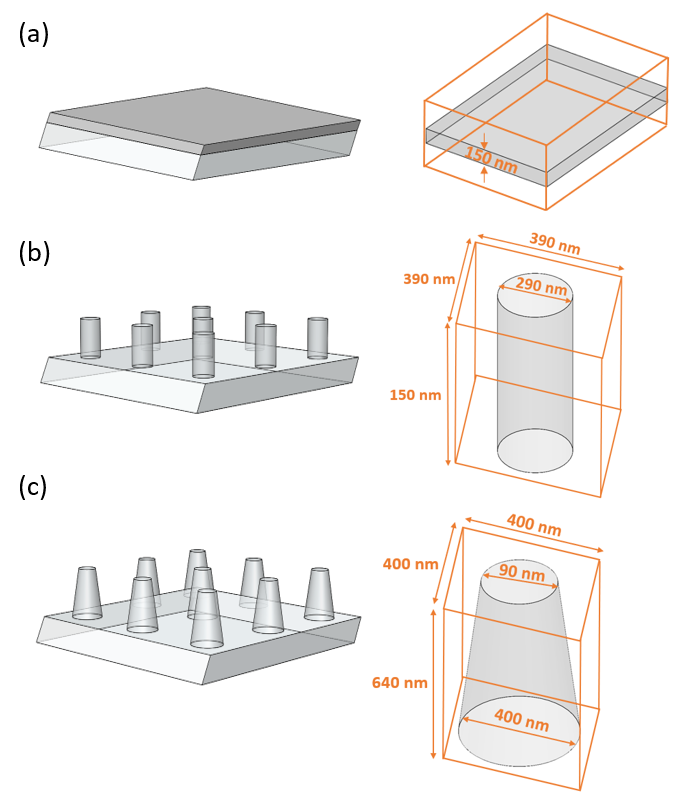
\includegraphics[height=3.5in]{Figures/figure1.png}
    %\caption{Caption}
    %\label{fig:Figure 1}
%\end{figure}

Recently, we utilized Bayesian learning optimization to determine the optimized antireflection properties of single layer thin film, nanowire arrays, and nanocone arrays, which are shown in Fig.~\ref{fig:Structures} \cite{Haghanifar:20}. 
%insert figure 1 here
The single layer thin film consists of a single dielectric 
with an an index of refraction of the geometric mean of glass and air or $n_1 = 1.21$ and thickness  $t = 120$ nm. 
% Normal reflection of 0.51
% reflection at 65 degrees of 5.05 
The nanowire array has a pitch $a = 390$ nm, a diameter of $d = 290$ nm, and a height of $h = 150$ nm.
%of 390 and 290 nm, respectively.  
%diameter of  
%.  
% normal reflection of .4745
% reflection at 65 degrees of 5.77
The nanocone has a pitch $a = 400$ nm, 
bottom diameter $d_{bot} = 400$ nm, top diameter $d_{top} = 90$ nm, and height $h = 640$ nm.
% normal reflection of 0.16
% reflection at 65 degrees of 1.25
\begin{figure}[H]
\vspace{-10pt}
 \centering
 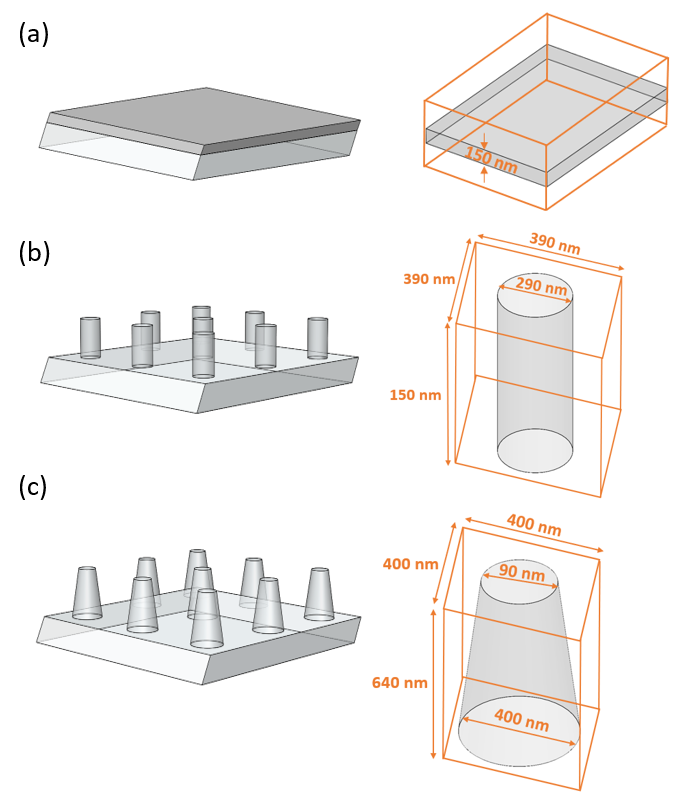
\includegraphics[width=10.5cm]{Figures/figure1.png}
\caption{Structures and dimensions of the (a) thin film, (b) nanowire, and (c) nanocone simulated in this study.}
 \label{fig:Structures}
 \end{figure}

We combine this with a simple model for studying available solar irradiance for different module orientations and latitudes
\cite{Sharma:21} to determine the annual enhancement of available solar irradiance with different types of antireflection coatings.  

%\commentPaul{Please create schematic of the different structures.  You can just modify the schematic we used before but give the exact dimensions.}



% The total solar module photon flux consists of both the direct beam and the diffuse components, 
% \begin{equation}
% \Phi_{Tm} = \Phi_{bn} \cos \theta + \frac{1 + \cos \beta}{2} \Phi_{d}   
% \end{equation}
where $\Phi_{bn}$ is the photon flux of the direct beam radiation and 
$\Phi_d$ is the diffuse isotropic sky photon flux.  
$\theta$ is the angle between the direct beam radiation on the module and the normal to
the module surface. $\beta$ is the solar module tilt.  
We assume the irradiance of the diffuse radiation is 10\% that of the direct beam radiation
% \begin{align}
% I_d = 0.1 I_{bn},
% \end{align}
as is the case with the AM1.5G and AM1.5D standard spectra. 

The direct beam spectral irradiance $F(\lambda)$ of arbitrary airmass $AM$ is 
\begin{equation}
F\_{bn} (\lambda) = F\_{AM0} (\lambda) \left [ \frac{F\_{AM1.5D} (\lambda)}{F\_{AM0} (\lambda)}  \right ] ^{ \left ( AM/1.5 \right )^{0.678}}
\end{equation}
where $F_{AM0}(\lambda)$
and $F_{AM1.5D}(\lambda)$ are 
the spectral irradiance of the AM0 and AM1.5D spectrum \cite{AM1p5}, respectively and $\lambda$ is the wavelength in vacuum. 
The power relationship is a  fit to empirical data \cite{Meinel:76}.
The direct beam irradiance of particular air mass may be obtained by integrating the spectral irradiance
%direct beam irradiance 
\begin{equation}
I\_{bn} = \int F\_{bn} (\lambda) d (\lambda) d (\lambda)
\label{eq:IAMDb}.
\end{equation}

The AM1.5G spectrum is assumed to follow the same scaling as AM1.5D and the diffuse radiation can be obtained from the difference between the two gobal spectral irradiance and the direct beam spectral irradiance:
\begin{align}
F_{d} (\lambda) = F_{AM0} (\lambda) 
 \left [ \frac{F_{AM1.5G} (\lambda)}{F_{AM0} (\lambda)}  \right ] ^ {\left ( AM/1.5 \right ) ^{0.678}} - 
F_{bn} 
\end{align}
%  \begin{align}
% F_{d} (\lambda) = F_{AM0} (\lambda) 
% \left \{
% \left \left [ \frac{F_{AM1.5G} (\lambda)}{F_{AM0} (\lambda)}  \right ] ^ {\left ( AM/1.5 \right ) ^{0.678}} - 
% \left [
% \frac{F_{AM1.5D} (\lambda)}{F_{AM0} (\lambda)}  \right ] ^ {\left ( AM/1.5 \right ) ^{0.678}}
% \right \}
% \end{align}
%  \begin{align}
% F_{d} (\lambda) = F_{AM0} (\lambda) \left [ \frac{F_{AM1.5G} (\lambda) - F_{AM1.5D} (\lambda)}{F_{AM0} (\lambda)}  \right ] ^ {\left ( AM/1.5 \right ) ^{0.678}}
% \end{align}
% where $F_{AM1.5G}(\lambda)$
% is 
% the spectral irradiance of the AM1.5G spectrum \cite{AM1p5}.


\begin{align}
I_{d} & = \int F_{d} (\lambda) d \lambda
\label{eq:IAMDb}.
\end{align}



The direct beam photon flux density is related to the spectral irradiance by
\begin{equation}
b_{bn} (\lambda) = \frac{F_{bn} (\lambda) \lambda} {h c}.
\end{equation}
\begin{equation}
b_{d} (\lambda) = \frac{F_{d} (\lambda) \lambda} {h c}.
\end{equation}
The photon flux is 
\begin{equation}
\Phi_{bn} = \int b_{bn} (\lambda)  d \lambda
\end{equation}
\begin{equation}
\Phi_{d} = \int b_{d} (\lambda) d \lambda
\end{equation}



The total photon flux incident on a module is the sum of the direct beam and diffuse components
\begin{equation}
\Phi_{Tm} = \Phi_{bn} \cos \theta + \frac{(1 + \cos \beta)}{2} \Phi_d
\end{equation}
The annual module incident photon flux is
\begin{align}
B_{mA} &= \frac{12}{\pi} \times 3600 \int_{0}^{365} \int_{-\omega_s} ^{\omega_s} \Phi_{Tm} d \omega d n %\\%\\
%I_{DA} (l) &= 2  \frac{12}{\pi}  \int_{-23.45 \degree}^{23.45 \degree} \int_{\cos^{-1} \left ( - \frac{ \sin(\delta)\sin( l)}{\cos(\delta)\cos(l)} \right ) } ^{\cos^{-1} \left ( - \frac{ \sin(\delta)\sin( l)}{\cos(\delta)\cos(l)} \right )} 1.353*0.7{^{AM (\omega, \delta, l)}}^{{0.678}} d \omega d \delta \\
%&=  \int_{-23.45 \degree}^{23.45 \degree} \int_{0 } ^{\cos^{-1} \left ( - \frac{ \sin(\delta)\sin( l)}{\cos(\delta)\cos(l)} \right )} 1.353*0.7{^{AM (\omega, \delta, l)}}^{{0.678}} d \omega d \delta
\end{align}
$\omega_s$ is the sunset hour angle,
\begin{align}
 \omega_s &= \cos^{-1} \left ( - \tan \phi \tan \delta \right ) 
\end{align}
and $-\omega_s$ is the sunrise hour angle.



% The direct beam photon flux is 
% \begin{equation}
% \Phi_{bn} = \int b_b (\lambda) d \lambda
% \end{equation}

% The daily direct beam photon flux is 
% \begin{equation}
% B_{bD}  = \frac{12}{\pi} \times 3600 \int_{-\omega_s}^{\omega_s} \int b_b (\lambda) d \lambda d \omega
% \end{equation}


 



% The annual average daily total module insolation is
% \begin{align}
% H_{Tm} = \frac{1}{365} \int_0^{365} \frac{12}{\pi} \int_{-\omega_s}^{\omega_s}  I_{Tm} d \omega d n    
% \end{align}
% %where $\omega$ is the hour angle.
% where $\omega_s$ is the sunset hour angle
% \begin{align}
%  \omega_s &= \cos^{-1} \left ( - \tan \phi \tan \delta \right ) 
% \end{align}
% and $-\omega_s$ is the sunrise hour angle.
% $\omega = 0$ at solar noon.  

The number of photons not reflected by the module is

\begin{equation}
b_{Tc} =  b_{bn}  \left [ 1 - R(\lambda, \theta, \gamma_i) \right ]  +  
 b_d \frac{1}{2 \pi } \int_{0}^{2 \pi} \int_{0}^{\pi/2 - \beta} \left ( \frac{1 + \cos \theta}{2} \right ) \left [ 1 - R(\lambda, \theta, \gamma_i)  \right ] d \theta d \gamma
\end{equation}

where $R(\lambda, \theta, \gamma_i)$ is the reflection spectra of the module/interface is a function of 
angle of incidence $\theta$, and injection azimuth angle $\gamma_i$. 
$\gamma_i = \gamma - \gamma_s$, where $\gamma$ is the module azimuth angle and $\gamma_s$ is the solar azimuth angle.  
The azimuth angle is defined so $0 \degree$ is south,   negative is east, and positive is west \cite{Duffie:13}.  
The total photon flux transmitted through the top glass is 
\begin{equation}
\Phi_{Tc} = \int b_{Tc} (\lambda) d \lambda
\end{equation}
The annual solar cell flux is 
\begin{equation}
B_{cA} = \frac{12}{\pi} \times 3600 \int_{0}^{365} \int_{-\omega_s} ^{\omega_s} \Phi_{Tc} d \omega d n 
\end{equation}
The annual module reflection is the portion of photons over an entire year that are lost due to 
reflection is 
%reflection
\begin{equation}
R_{mA} = \frac{1 - B_{cA} }{B_{mA}}.
\end{equation}





The reflection spectra of various antireflection structures is shown in 
Fig.~\ref{fig:ARspectra}.
The reflection is shown as a function of wavelength along the radius and incidence angle $\theta$ in the circumferential direction.  The reflection is shown for (a) bare glass, (b) thin film, (c) nanowire array, and (d) nanocone array.  
The reflection spectra shown is averaged for both TE and TM polarized light and over the incident azimuth angles $\gamma_i$.
The integrated reflection as a function of incidence angle $\theta$ is shown in 
Fig.~\ref{fig:ARspectra}(b).  The reflection spectra is integrated over wavelengths from 280 to 1200 nm.  

\begin{figure}[H]
\vspace{-10pt}
 \centering
 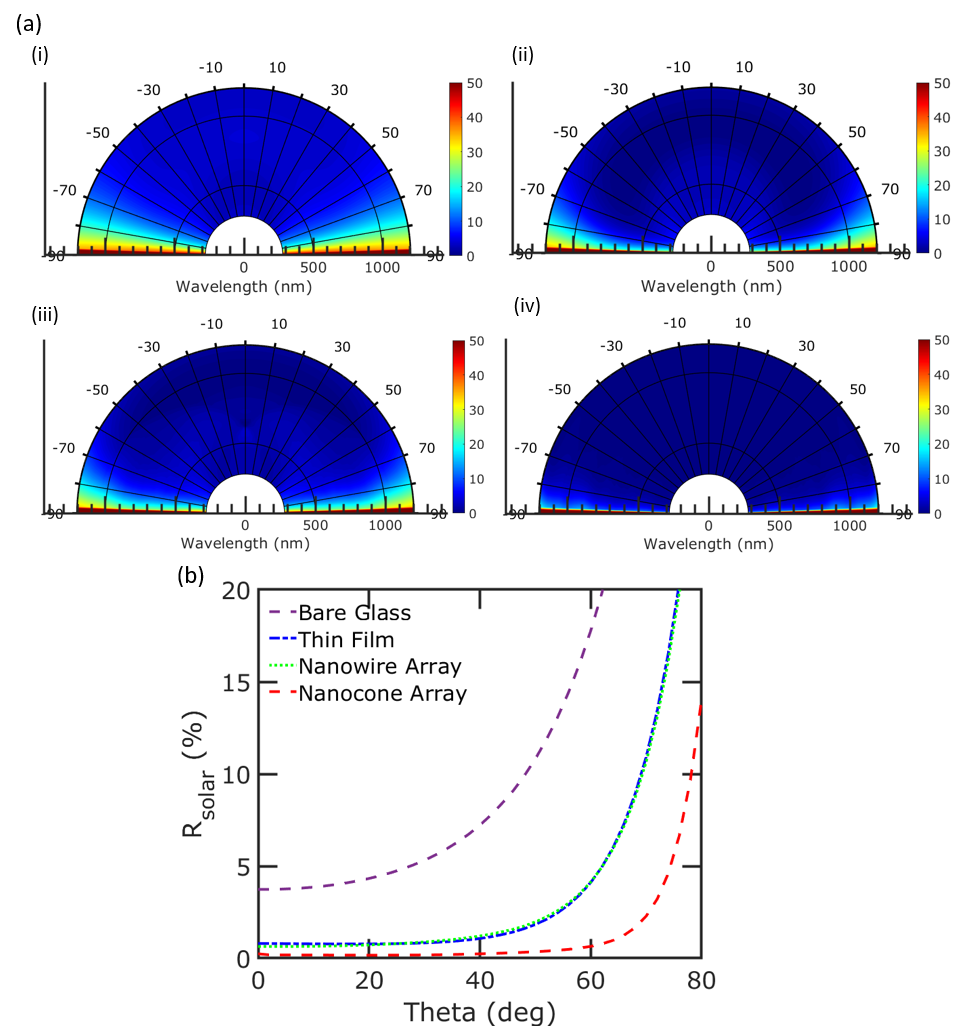
\includegraphics[width=13.5cm]{./Figures/figure2.png}
\caption{Reflection spectra of different structures.  (a) Reflection spectra as a function of incidence angle $\theta$ for (i) bare glass, (ii) thin film, (iii) nanowire array, and (iv) nanocone array.  
(b) Integrated solar reflection as a function of incidence angle.}
 \label{fig:ARspectra}
 \end{figure}






% where the air mass $AM$ is defined as 
% \begin{equation}
% AM (\omega, \delta, \gamma_s) = \frac{1}{cos\left [ \theta_z (\omega, \delta, \gamma_s) \right ]}.
% \end{equation}

% $\theta_z$ is the zenith angle of the sun, 
% $\omega$ is the hour angle, and $\delta$ is declination angle, and $\gamma$ is the module angle.
%whereωis the hour angle and $\delta$ is the %latitude.
%where 






%% The Appendices part is started with the command \appendix;
%% appendix sections are then done as normal sections
%% \appendix

%% \section{}
%% \label{}

%% If you have bibdatabase file and want bibtex to generate the
%% bibitems, please use
%%
%%  \bibliographystyle{elsarticle-num} 
%%  \bibliography{<your bibdatabase>}

%% else use the following coding to input the bibitems directly in the
%% TeX file.

%\begin{thebibliography}{00}
%
%%% \bibitem{label}
%%% Text of bibliographic item
%
%\bibitem{}

\section{Data Availability}

All python code used for the model to generate the figures in the manus-cript can be found in the following Github repository: \\ \url{https://github.com/pleu/LAMPsolar}.

\section{Acknowledgements}
This work was supported by the National Science Foundation [grant number 1930582].

\bibliographystyle{elsarticle-num}
\bibliography{LAMPPapers,AllRefs}


%\end{thebibliography}
\end{document}
\endinput
%%
%% End of file `elsarticle-template-num.tex'.
